\chapter{Tools And Scripts}


















\section{mmorpdnd.py}

\subsection{Purpose}

This script serves as the backbone for an array of automatic linking and logistical features within MMORPDND. These functionalities typically operate on all files, encompassing crucial elements such as the generation of directories, HTML index files at the directory summits, establishment of uniform headers and navigation for all HTML documents, seamless interlinking between files, refinement of both HTML and CSS code, and an array of additional capabilities. When ran, this script will perform the following actions in the following order:

\begin{enumerate}
	\item Create Directory Structures if not already existing.
	\item Create index files for each directory.
	\item Update each index file to link to all files and images within the directory.
	\item Update the headers of all html files to the template html header.
	\item Update the navigation of all html files to the template navigation html.
	\item Search and hyperlink all words found in all html files to the appropriate html file whose name matches the words found.
	\item Beautify the code.
\end{enumerate}







\subsection{Use}

The mmorpdnd.py script can be ran as a gui window or using the command line options. The two main features are `test' and `update'. The `test' feature will create fake files and then perform the update command on them. This is useful for testing if the features and newly added features are working properly. The `update' feature will perform a combination of tasks which updates all appropriate files to do the steps mentioned in the list above.

\subsubsection{GUI}

\begin{figure}[h]
	\centering
	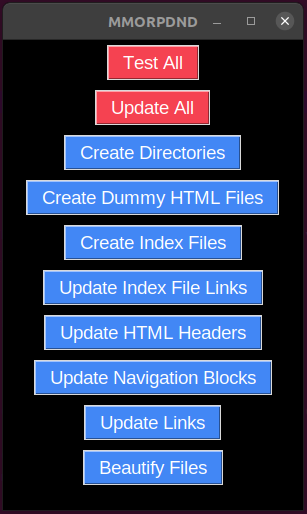
\includegraphics[width=0.5\textwidth]{images/mmorpdnd_gui.png}
	\caption{The MMORPDND Main GUI}
	\label{fig:mmorpdnd_gui}
\end{figure}

The GUI window is somewhat self explanatory. The two main features are represented by red buttons - the `test` and `update` features. There are also other buttons to simple perform and of the individual tasks using the appropriately associated button.

\subsubsection{Command Line}

The MMORPDND application supports some command line features.

\begin{lstlisting}
usage: mmorpdnd.py [-h] [-t] [-u]

MMORPDND Tools and apps.

optional arguments:
	-h, --help    show this help message and exit
	-t, --test    Runs the test-all feature then exit.
	-u, --update  Runs the update-all feature then exit.
\end{lstlisting}





























\section{templates/creator.py}



\subsection{Purpose}

The creator tool is a practical solution for converting basic template text files into functional HTML pages. It takes care of the technical aspects by automatically creating HTML files and filling in missing details, like character stats or other content. The tool understands the structure of your template files, recognizes placeholders, and replaces them with accurate data. Whether you're building character profiles, story summaries, or any content with consistent formatting, this tool ensures your HTML documents are correctly formatted and ready for use. It simplifies the process, letting you focus on content creation while it handles the conversion from templates to HTML.

\subsection{Use}

The creator tool is a powerful tool that contains many subtle features. It is important to understand these subtleties before using the tool and therefore I encourage the reader to read this enture section before use. 

\subsubsection{GUI}

\begin{figure}[h]
	\centering
	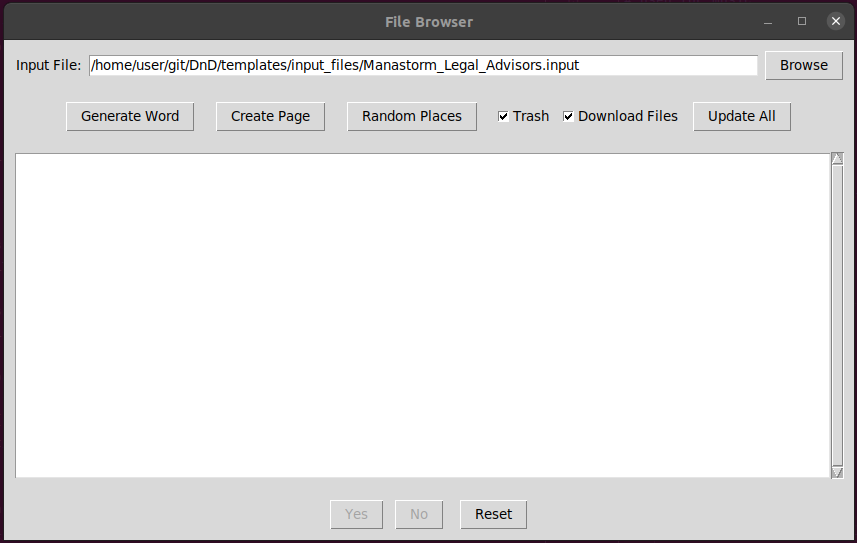
\includegraphics[width=0.9\textwidth]{images/creator_gui.png}
	\caption{The MMORPDND Main GUI}
	\label{fig:creator_gui}
\end{figure}

The main GUI of the creator tool has a few components. These include text boxes, buttons, and check boxes. 

The ``Input File" text box field is used to specify the input file that is to be processed by the tool. This file can be an `.input', `.char' or `.names' file. Ensure the file is in the proper format (see below sections) or unexpected behavior may occur. The `Browse' button is used to open a file explorer window for selecting a file and will automatically populate the ``Input File" text field when a file is selected. The large text box in the center of the GUI is where output generated from the tool as well as status messages are displayed.

The ``Generate Word" button is used for random word generation. This feature takes a list of words (whether names, places, or other) and generates a similar random word using the data in the input `.names' file. This is explained in more detail later in section \ref{section .names}. The ``Create Page'' button is used to generate an HTML file based on a `.input' or `.char' file and is explained in more details in the following sections. the ``Random Places'' file is used to generate place names based on an input `.names' file along with a `.list' file. These are explained mroe in later sections. The ``Yes", ``No", and ``Reset" buttons are used when user input is asked for. The ``Update All" button performs the same functions as the mmorpdnd.py update function (see the previous sections).

The ``Trash" checkbox will determine if processed files will be moved to the trash folder after processing and if duplicate files are to be deleted. Typically, the user will want this to be checked, but it is useful to leave unchecked for testing and if files will be processed multiple times. The ``Download Files" button determines if music files should be downloaded when `.input' files containing a dnd-music section are processed (this is explained mroe in later sections).

\subsubsection{Input Files (.input)}

The input files are essentially just text files with the file extension `.input'. The main feature of the creator.py tool is to read in these input files, parse them, and generate the appropriate html files from them. These input files must follow a strict formatting but offer a few various helpful features. The name and main heading of the generated HTML file will be created based on the name of the input file (underscores will be replaced by spaces for the heading). Each line of the input file represents a 'section' of the html file that will be generated. Each line follows the following format:
\begin{lstlisting}
Heading Text[type]=Information text
\end{lstlisting}
The "Heading Text" is what will appear as the header for that html section. The "type" value is what determines the properties of this section and how it is interpreted by the creator tool. The "Information text" is the actual information for that section. The only exception to this rule is the first line which defines the "folder" that the html file generated from the input file will be placed into. This "folder" line is special in that it has no type and the creator tool will recognize the folder keyword and store this information separately. This folder line must be formatted as follows:
\begin{lstlisting}
folder=path/to/where/I/want/my/generated/file
\end{lstlisting}
The various types determine the formatting and decoding of the input file, and each type has small subtleties. The various types are
\begin{enumerate}
	\item dnd-image: This type is used to display an image or multiple images.
 	\item dnd-list: This is used to display a list of items.
 	\item dnd-info: This is used for general information and sections. It also supports listing information between paragraphs.
  	\item dnd-music: This is a section for storing various music for the regions.
\end{enumerate}

\subsubsection{dnd-image type}

The \textbf{dnd-image} type is used to display images specific to the file. The information text must contain three parameters separated by a semi-colon delimeter. These parameters are \textbf{img/image-name.jpg;image source;image caption}. The first parameter is simply the location of the image and the image name. These are typically placed in `templates/img'. The second is the source of the image, this is simply a string but is there to keep all images properly sourced. The third is a caption that will be displayed with an image. This caption is also a string and can be whatever the user desires. As an example, here's a proper dnd-image block (see figure \ref{fig:dnd-image-fig}):

\begin{lstlisting}
Coconatus Marmotta[dnd-image]=img/coconatus_marmotta.jpg;Created by Bing AI image creator;Coconatus Marmotta.
\end{lstlisting}

\begin{figure}[h]
	\centering
	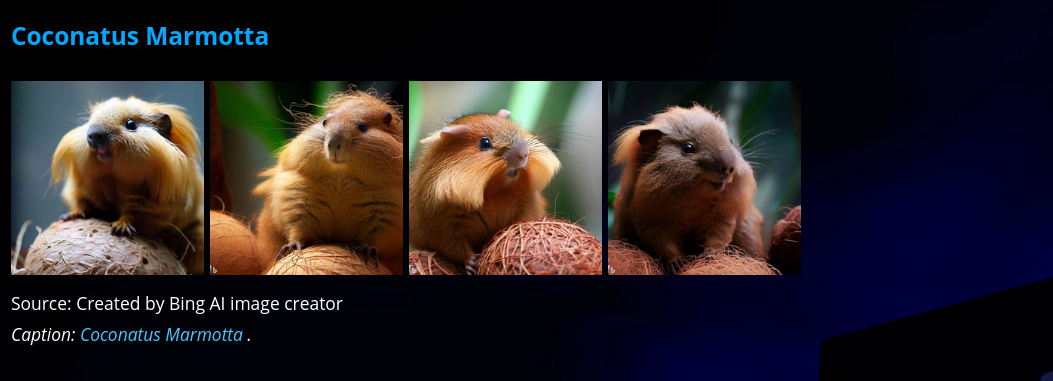
\includegraphics[width=0.8\textwidth]{images/dnd-image-section.png}
	\caption{A dnd-image section generated using 4 images.}
	\label{fig:dnd-image-fig}
\end{figure}

One unique feature of this is that if the image name does not exist (i.e. `img/coconatus\_marmotta.jpg'), the tool will append a ` (1)' to the name and search again (i.e. `img/coconatus\_marmotta (1).jpg'). If this new name is found, the tool will search for image names with the index incremented and include all such images (i.e. `img/coconatus\_marmotta (2).jpg', `img/coconatus\_marmotta (3).jpg', etc) in the output html block.  

\subsubsection{dnd-list type}

The \textbf{dnd-list} type is used to display a simple list of items. The information text must contain one or more parameters separated by a semi-colon delimeter. As an example, here's a proper dnd-list block (see figure \ref{fig:dnd-list-fig}):

\begin{lstlisting}
Landmarks and Other Features[dnd-list]=Talleril: A small island far off the coast of Alderpine.;Enthilma: A small island off the coast of Alderpine.;Lomelindei: The large world tree deep within Alderpine.
\end{lstlisting}

\begin{figure}[h]
	\centering
	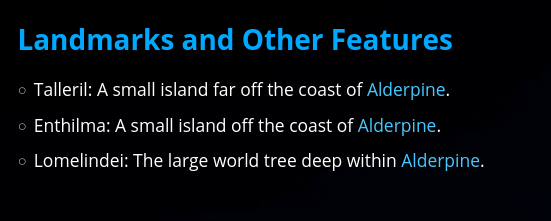
\includegraphics[width=0.6\textwidth]{images/dnd-list-section.png}
	\caption{A dnd-list section.}
	\label{fig:dnd-list-fig}
\end{figure}

\subsubsection{dnd-info type}

The \textbf{dnd-info} type is used to display a section of text. The information text must contain one or more parameters separated by a delimeter. The delimeter for this type will define the format of the sections within this text. For writing normal paragraphs, simple use a semi-colon (`;') delimeter. The semi-colon delimeter will make the next parameter appear as a normal paragraph. As an example, here's a proper dnd-info block (see figure \ref{fig:dnd-info-fig-01}):

\begin{lstlisting}
Some Paragraphs[dnd-info]=This is a paragraph.;This is a second paragraph.;This is a third paragraph.;etc...
\end{lstlisting}

\begin{figure}[h]
	\centering
	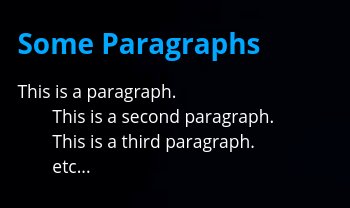
\includegraphics[width=0.6\textwidth]{images/dnd-info-section-01.png}
	\caption{A dnd-info section with only paragraphs. Note that the first paragraph will not be indented but all subsequent ones will be.}
	\label{fig:dnd-info-fig-1}
\end{figure}

To add in a list element between paragraphs, you can use a semi-colon and dash (`;-') delimeter. The `;-' delimeter will tell the creator tool that a list has began and the it will use all subsequential parameters with a preceeding `;-' delimeter as the list items until a different delimeter is entered or there is no more parameters to read in. As an example, here's a proper dnd-info block (see figure \ref{fig:dnd-info-fig-02}):

\begin{lstlisting}
Some Paragraphs and a List[dnd-info]=This is a paragraph.;-Here's a list item 1.;-Here's another list item;-Here's a third list item;Here's an ending paragraph.
\end{lstlisting}

\begin{figure}[h]
	\centering
	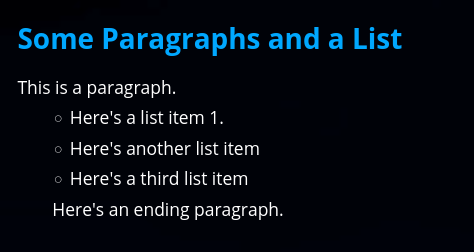
\includegraphics[width=0.6\textwidth]{images/dnd-info-section-02.png}
	\caption{A dnd-info section with a paragraph followed by a list, followed by a paragraph.}
	\label{fig:dnd-info-fig-2}
\end{figure}

To add a subsection, you can use the semi-colon followed by an asterik (`;*') as the delimeter. This delimeter has a somewhat special formatting in that there needs to be a second asterik to mark the end of the subsection heading. For example, `;*heading text*normal content text'. The `heading text' will display as a subheading, while the `normal content text' will be the main content under that subsection. As an example, here's a proper dnd-info block (see figure \ref{fig:dnd-info-fig-03}):

\begin{lstlisting}
Some subsections[dnd-info]=Here is a paragraph;*Subheading*Some text;Here's another paragraph;*Subheading 2*More text;Here's an ending paragraph.
\end{lstlisting}

\begin{figure}[h]
	\centering
	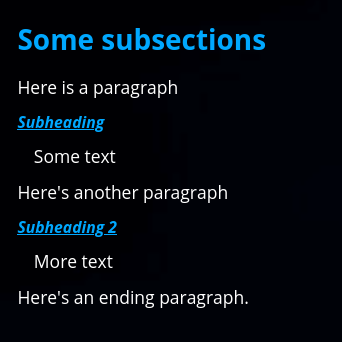
\includegraphics[width=0.6\textwidth]{images/dnd-info-section-03.png}
	\caption{A dnd-info section with some paragraphs and two subsections.}
	\label{fig:dnd-info-fig-3}
\end{figure}

\subsubsection{dnd-music type}

The \textbf{dnd-music} type is used to display a simple list of music items. The information text must contain one or more parameters separated by a semi-colon delimeter. Currently, this is primarily designed to work with youtube links. Given a simple youtube link, the code will find the name of the video and use that as the list information as well as keeping a link to the video itself. If the ``Download Links" checkbox in the GUI is enabled, the files will be downloaded as mp3 files and the folder next to the list item will be hyperlinked to the local file. These files will be located in a music folder. As an example, here's a proper dnd-music block using fake URL's (see figure \ref{fig:dnd-music-fig})::

\begin{lstlisting}
Music And Ambiance[dnd-music]=https://youtube_link_1;https://youtube_link_2;https://youtube_link_3
\end{lstlisting}

\begin{figure}[h]
	\centering
	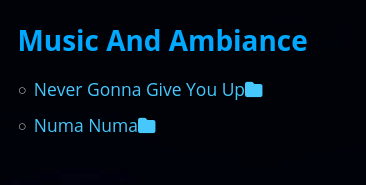
\includegraphics[width=0.6\textwidth]{images/dnd-music-section.png}
	\caption{A dnd-music section with two songs linked to.}
	\label{fig:dnd-music-fig}
\end{figure}


\subsubsection{Example Input File}

For example input files, you can look inside the templates/trash folder. This is where input files get placed after they are finished processing. The following is an example input file with an example of many different elements. The associated image files `foobar.jpg', `foobars (1).jpg' and `foobars (2).jpg' should be located in the templates/img folder for the below file to process correctly.

\begin{lstlisting}
folder=items

A Single Image[dnd-image]=img/foobar.jpg;Created by Someone;A foobar image.

Information Section[dnd-info]=Here is a paragraph of text.;Here is a second paragraph.

Information Section With Smaller Headers[dnd-info]=Here is a paragraph of text.;*Small Header* Here is a second paragraph.

A List Of Items[dnd-list]=item A; Item B; Item C; Item D

Multiple Images[dnd-image]=img/foobars.jpg;Created by Someone;Multiple foobar images.

Information Section with List[dnd-info]=Here is a paragraph of text followed by a list;-List_item_A;-List_item_B;-List_item_C;Followed by a paragraph.

Music And Ambiance[dnd-music]=https://youtube_link_1;https://youtube_link_2;https://youtube_link_3
\end{lstlisting}

The above file will create a file in the `items' folder found in `campaign/items'. The file will start with a header "A Single Image", where the foobar.jpg image is displayed. A caption of "A foobar image." will be under the image. Next will be a heading "Information Section" That has two paragraphs. Next a similar section with a header "Information Section With Smaller Headers", a paragraph, then a smaller header "Small Header", followed by another paragraph. Next, another heading "A List Of Items" with 4 items in the list. Following this, a "Multiple Images" heading with 2 images `foobars (1).jpg' and `foobars (2).jpg'\footnote{If an image is not found, it will automatically search for files with that image name with an appended (1), (2), (3),... If `(1)' is found, this image will be used and the number incrememted until no other images are found.} with a caption "Multiple foobar images." Next, another heading ``Information Section with List", with a paragraph, a list, and then another paragraph. Finally, a heading "Music And Ambiance" with links to three youtube videos. If the "download links" checkbox is enabled, these video's will be downloaded as mp3 files and the fodler icon will link to the local files.






\subsubsection{Character Files (.char)}

The character files are text files with the ".char" extension. These are a special type of input file that generates an html page specific for DnD character information. This was actually designed before the more general input file formatting outlined in the sections above and therefore lacks some of the versatility and extra features that can be included in the input files. Nevertheless, the character format creates an html page that should more than suffice for any npc characters and has many of its own unique features and capabilities. The .char file contains lines that define the various elements of a character. These lines to not currently support the types that are supported with the input files. Each line has a specific output format in the generated html file based on a template and the information itself. Some lines in the file are required while others are optional. The required lines must be present for the character file generated to be completed, while the optional lines will automatically be randomized and generated in the event that they are missing. Eahc line of the character file must be formatting in the following way:
\begin{lstlisting}
Keyword = Value
\end{lstlisting}
The "Keyword" is used by the creator tool to determine which type of information is being input, and the "Value" is the value of the information. For example "level = 3" would let the creator know that the character level is 3, and it will use that information appropriately.

Once the character file is appropriately filled out and created, it should be saved/placed in the templates/input\_files folder for processing by the creator tool just like the .input files. The creator tool will search the templates/img folder for any image references within the character files.






\subsubsection{Required Keywords}

The required keywords for a character file are the following:
\begin{enumerate}
	\item folder: This defines the folder that the output html character file will be placed. This should be a valid file path to a folder.
	\item name: This defines the name of the character.
	\item image: This is an image for the character. This should be just the image file name and extension (no path) and the image itself should be placed in the "templates/img" folder for automatic detection.
	\item class: This defines the DnD class. This must be a valid class from the following list:
		\begin{multicols}{3}
		    \begin{itemize}
		        \item barbarian
		        \item bard
		        \item cleric
		        \item druid
		        \item fighter
		        \item monk
		        \item paladin
		        \item ranger
		        \item rogue
		        \item sorcerer
		        \item warlock
		        \item wizard
		    \end{itemize}
		\end{multicols}
	\item abilities: The abilities of the character. This field is a list and should be entered using a comma (`,') as the delimeter.
	\item equipment: The equipment of the character. This field is a list and should be entered using a comma (`,') as the delimeter.
	\item proficiencies: These are the proficiencies of the character. This field is a list and should be entered using a comma (`,') as the delimeter. The proficiency bonus will automatically be calculated based on level and applied to proficiencies.
	\item information: General information and description of the character.
\end{enumerate}

The above list of keywords are all required and if they are missing or ill-formatted, unexpected behavior can occur.






\subsubsection{Optional Keywords}

The optional keywords for a character file are the following:
\begin{enumerate}
	\item level: This is the level of the character. If the level is not defined, it will default to 1. This must be an integer.
	\item hp: This will be generated automatically if not included based on the character class, level, and constitution\footnote{The constitution value is automatically generated based on the character class and level if not included.} value.
	\item ac: The Armor class value.
	\item size: The size of the character.
	\item type: The type of the character (creature, humanoid, animal, etc)
	\item alignment: The alignment of the character.
	\item speed: The speed of the character.
	\item resistances: The resistances the character has (if any).
	\item immunities: The immunities the character has (if any)
	\item senses: The senses. A ", Passive Perception: \#" will automatically be appended to this value based on a calculated passive perception.
	\item languages: Languages of the character.
	\item race: The race of the character.
	\item background: The background of the character.
	\item strength: This represents the character's physical strength and ability to exert force. This must be an integer.
	\item dexterity: This represents the character's agility, reflexes, and fine motor skills. This must be an integer.
	\item constitution: This measures the character's health, stamina, and resistance to illness and fatigue. This must be an integer.
	\item intelligence: This reflects the character's mental acuity, memory, and problem-solving skills. This must be an integer.
	\item wisdom: This represents the character's perception, intuition, and common sense. This must be an integer.
	\item charisma: This measures the character's charm, persuasion, and ability to influence others. This must be an integer.
	\item notes: Notes to add about the character that aren't contained in the `information' section.
\end{enumerate}

It is recommended to include all values in the character file and just use "None" for any string values that are not needed. This will prevent any un-expected bugs. Many of the values replace a string in a template file based on the values input, so if they are not specified, a correlated `search string' will appear in the final html file that serves as a placeholder for the information.






\subsubsection{Example Character File}

For example character files, you can look inside the templates/trash/chars folder. This is where input files get placed after they are finished processing. The following is an example character file. The associated image file foobar.jpg should be located in the templates/img folder for the below file to process correctly.

\begin{lstlisting}
folder = characters/player
name = fooBar
ac = 16 (natural armor)
hp = 84
level = 13
size = small
type = humanoid
alignment = neutral good
speed = 30 ft.
resistances = None
immunities = None
senses = Darkvision 60ft
languages = Common, Elvish
image = foobar.jpg
race = Fooling
class = wizard
background = Barber
strength = 15
dexterity = 13
constitution = 18
intelligence = 22
wisdom = 4
charisma = 14
abilities = basic attack: A basic attack with nothing special; prestidigitation
equipment = torch; small sword, a potato
proficiencies = strength, acrobatics, history
information = This is some info for foobar, the template character.
notes = No notes needed for template dude.
\end{lstlisting}

Once created, the file should be placed in the templates/input\_files folder and then processed via the creator.py tool.










\subsubsection{Name Files (.names) \label{section .names}}

SECTION IN PROGRESS!








\subsubsection{List Files (.list) \label{section .list}}

SECTION IN PROGRESS!













\subsubsection{Command Line}

The creator application does NOT currently support command line features.

